\section{Implementation Details}\label{sec:Implementation}

The chaincode is written in Golang and provides all contracts needed to proceed with traceability in the application. All contracts for use in chaincode must implement the interface \textit{contractapi.ContractInterface}. 

The first step is to create a JSON config file providing all information about these three items. A configuration file includes \textit{assetId}, a list of actors, and a list of ordered steps. The chaincode processes this file through  \textit{initLedger} and \textit{createNewAsset} functions. A template for the config file can be found in appendix \ref{app:template}.

Front-end WebApp enables users to define settings through a Configuration Page, adding these to the configuration file, as shown in Figure~\ref{fig:create_asset_4}. Assets, asset items, steps, and actors are described in appendix \ref{app:structs}. There are create methods for each one,  responsible for creating an instance of these \textit{structs} and save the state into the blockchain. Query methods are responsible for interact with the information of any item in the blockchain.

The chaincode \textit{main} function invokes the \textit{initLedger} function, reads the configuration files, and raises the platform enabling users to interact with the blockchain via exposing its API.

When creating an asset item, an \textit{AssetItemId} is generated. Each entity in the chain will have its unique entity ID and timestamp when processing the transaction. By querying \textit{AssetItemId}, the user can easily track the current transaction information and status. Finally, completed all steps, the blockchain will update \textit{deliverDate} and mark the status as completed once the last actor (generally the consumer) has received the order. The \textit{CreateAsset} function is detailed in appendix \ref{app:CreateAsset}.


\textit{MoveAssetItem} is the method to update an asset item when moved from one step to another. It updates the \textit{CurrentOwnerId}, the \textit{ProcessDate}, information about prices, and many other details of the transactions by the key/value map \textit{aditionalInfo}. Its details are in appendix \ref{app:MoveAssetItem}.

\textit{TrackAssetItem} is the method responsible for tracking an asset item. It returns the children's tree of the given element and its ancestors from the beginning of the Supply chain. This method uses the function \textit{getChildenTree} to get the current item's children nodes. Appendix \ref{app:TrackAssetItem} contains its implementation.

For audit purposes, some methods were implemented to get info about the blocks and transactions stored in the ledger. These are the methods: \textit{getBlockByTxID, getChainInfo, getBlockByHash, getBlockByNumber,} and \textit{getTransactionByID}. Appendix \ref{app:auditMethods} contains their implementation.

%htbp
\begin{figure}[ht]
\begin{center}
  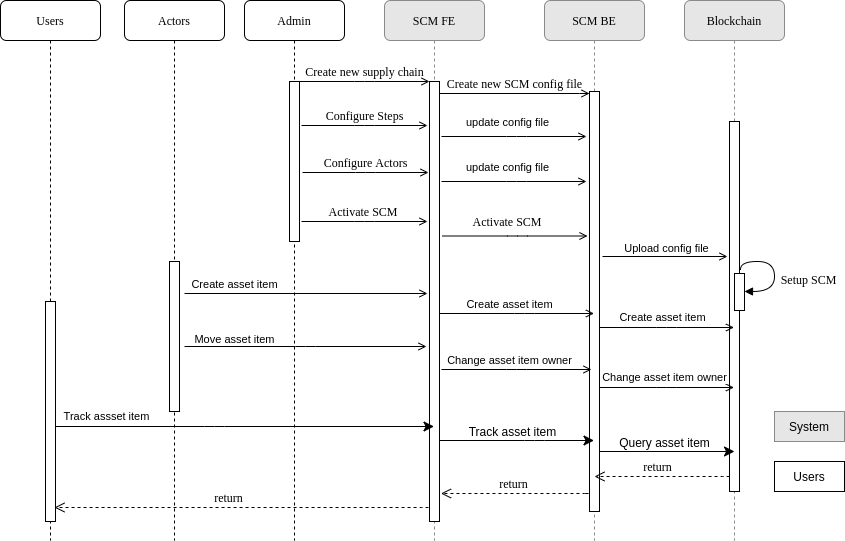
\includegraphics[scale=0.5]{images/SequenceDiagram.png}
\caption{SCM User flow}
\label{fig:sequenceDiagram}
\end{center}
\end{figure}

Figure~\ref{fig:sequenceDiagram} shows the interaction flow from users with the Arion platform. Initially, an admin persona creates and configure the SCM, adding information about the steps and the users. After that, the admin can activate this SCM, and from that point, the actors can interact with the SCM to provide information about an asset item and also move this asset item through the supply chain. From that point, any user can track an asset item to get information about the required goods.

The backend gateway exposes all the endpoints shown in table \ref{table:endpoints}. These endpoints are integrated with the frontend and can be used in future work to integrate with a mobile app or an external application.


\begin{table}[htb]
\centering
\caption{Backend endpoints}
\label{table:endpoints}
    \begin{center}
    \begin{tabular}{|l|p{4.5cm}|p{7.664cm}|}
        \hline 
        \thead{Verb} & \thead{URI} & \thead{Description}\\
        \hline 
        \cellcolor{cyan}\textbf{Actors}  & \cellcolor{cyan}\textbf{} & \cellcolor{cyan}\textbf{} \\
        \hline 
        POST & /actors & creates a new actor\\
        \hline 
        GET & /actors & retrieves the actors' list\\
        \hline 
        PUT & /actors/:id & updates an existing actor\\
        \hline 
        GET & /actors/:id & retrieves an existing actor\\
        \hline 
        DELETE & /actors/:id & removes an existing actor\\
        \hline 
        \cellcolor{cyan}\textbf{Steps}  & \cellcolor{cyan}\textbf{} & \cellcolor{cyan}\textbf{} \\
        \hline 
        POST & /steps & creates a new step\\
        \hline 
        GET & /steps & retrieves the steps' list\\
        \hline 
        PUT & /steps/:id & updates an existing step\\
        \hline 
        GET & /steps/:id & retrieves an existing step\\
        \hline 
        DELETE & /steps/:id & removes an existing step\\
        \hline 
        \cellcolor{cyan}\textbf{Asset Items}  & \cellcolor{cyan}\textbf{} & \cellcolor{cyan}\textbf{} \\
        \hline 
        POST & /asset-items & creates a new asset item\\
        \hline 
        GET & /asset-items & retrieves the asset items' list\\
        \hline 
        PUT & /asset-items/:id & updates an existing asset item\\
        \hline 
        GET & /asset-items/:id & retrieves an existing asset item\\
        \hline 
        DELETE & /asset-items/:id & removes an existing asset item\\
        \hline 
        POST & /asset-items/:id & moves an asset item through the SCM\\
        \hline 
        GET & /asset-items/track/:id & tracks an asset item through the SCM\\
        \hline
        \cellcolor{cyan}\textbf{Assets}  & \cellcolor{cyan}\textbf{} & \cellcolor{cyan}\textbf{} \\
        \hline 
        POST & /assets & creates a new asset\\
        \hline 
        GET & /assets & retrieves the assets' list\\
        \hline 
        PUT & /assets/:id & updates an existing asset\\
        \hline 
        GET & /assets/:id & retrieves an existing asset\\
        \hline 
        DELETE & /assets/:id & removes an existing asset\\
        \hline 
        \cellcolor{cyan}\textbf{Audit}  & \cellcolor{cyan}\textbf{} & \cellcolor{cyan}\textbf{} \\
        \hline
         GET & /blocks/:number & Return the block specified by block number\\
        \hline 
         GET & /blocks/hash/:hash & Return the block specified by block hash\\
        \hline 
         GET & /blocks/tx-id/:tx-id & Return the transaction specified by Transaction ID\\
        \hline 
         GET & /transactions:id & Return the transaction specified by ID\\
        \hline 
         GET & /chain & Return a blockchain Info object marshalled in bytes\\
        \hline 
    \end{tabular}
    \end{center}
\end{table}